\cleardoublepage\chapter{Graphs}\label{chap:plots}
This appendix contains plots and figures that are to voluminous to be placed anywhere else.

\section{Fast Fourier Transform of vehicle signatures}
The sampling frequency in all figures in this section is 25~Hz. The of the simulated data FFT has been plotted for all vehicle types used in this thesis and for all three axes. The sensor was placed at the side of the road.

% XXXXXXXXXXXXXXXXXXXXXXXXXXXXXXXX
\begin{subfigures}
\begin{figure}[thb]
 \centering
 \begin{minipage}{0.45\linewidth}
 	\centering
 	% generated by laprint.m
%
% \begin{psfrags}%
% \psfragscanon%
%
% text strings:
\psfrag{s02}[b][b]{\fontsize{8}{12}\fontseries{m}\mathversion{normal}\fontshape{n}\selectfont \setlength{\tabcolsep}{0pt}\begin{tabular}{c}FFT $\hat{x}$-axis - Passenger car\end{tabular}}%
\psfrag{s03}[t][t]{\fontsize{8}{12}\fontseries{m}\mathversion{normal}\fontshape{n}\selectfont \setlength{\tabcolsep}{0pt}\begin{tabular}{c}Frequency / $f_s$\end{tabular}}%
\psfrag{s04}[b][b]{\fontsize{8}{12}\fontseries{m}\mathversion{normal}\fontshape{n}\selectfont \setlength{\tabcolsep}{0pt}\begin{tabular}{c}$\vert{}Y(f)\vert{}/1\cdot{}10^{-6}$\end{tabular}}%
%
% axes font properties:
\fontsize{6}{8}\fontseries{m}\mathversion{normal}%
\fontshape{n}\selectfont%
%
% xticklabels:
\psfrag{x01}[t][t]{$-0.5$}%
\psfrag{x02}[t][t]{$-0.4$}%
\psfrag{x03}[t][t]{$-0.3$}%
\psfrag{x04}[t][t]{$-0.2$}%
\psfrag{x05}[t][t]{$-0.1$}%
\psfrag{x06}[t][t]{$0$}%
\psfrag{x07}[t][t]{$0.1$}%
\psfrag{x08}[t][t]{$0.2$}%
\psfrag{x09}[t][t]{$0.3$}%
\psfrag{x10}[t][t]{$0.4$}%
\psfrag{x11}[t][t]{$0.5$}%
%
% yticklabels:
\psfrag{v01}[r][r]{$0$}%
\psfrag{v02}[r][r]{$0.01$}%
\psfrag{v03}[r][r]{$0.02$}%
\psfrag{v04}[r][r]{$0.03$}%
\psfrag{v05}[r][r]{$0.04$}%
\psfrag{v06}[r][r]{$0.05$}%
\psfrag{v07}[r][r]{$0.06$}%
\psfrag{v08}[r][r]{$0.07$}%
\psfrag{v09}[r][r]{$0.08$}%
\psfrag{v10}[r][r]{$0.09$}%
%
% % Figure:
% \resizebox{6cm}{!}{\includegraphics{fft-car-x.eps}}%
% \end{psfrags}%
%
% End fft-car-x.tex

	\includegraphics[width=1\linewidth]{images/fft-car-x}
  	\caption[FFT $\hat{x}$-axis - Passenger car]{FFT $\hat{x}$-axis - Passenger car.\\}
  	\label{fig:fft-car-x}
 \end{minipage} \hfill
 \begin{minipage}{0.45\linewidth}
 	\centering
  	% generated by laprint.m
%
% \begin{psfrags}%
% \psfragscanon%
% %
% text strings:
\psfrag{s02}[b][b]{\fontsize{8}{12}\fontseries{m}\mathversion{normal}\fontshape{n}\selectfont \setlength{\tabcolsep}{0pt}\begin{tabular}{c}FFT $\hat{x}$-axis - Passenger car\end{tabular}}%
\psfrag{s03}[t][t]{\fontsize{8}{12}\fontseries{m}\mathversion{normal}\fontshape{n}\selectfont \setlength{\tabcolsep}{0pt}\begin{tabular}{c}Frequency / $f_s$\end{tabular}}%
\psfrag{s04}[b][b]{\fontsize{8}{12}\fontseries{m}\mathversion{normal}\fontshape{n}\selectfont \setlength{\tabcolsep}{0pt}\begin{tabular}{c}$\vert{}Y(f)\vert{}/1\cdot{}10^{-6}$\end{tabular}}%
%
% axes font properties:
\fontsize{6}{8}\fontseries{m}\mathversion{normal}%
\fontshape{n}\selectfont%
%
% xticklabels:
\psfrag{x01}[t][t]{$-0.5$}%
\psfrag{x02}[t][t]{$-0.4$}%
\psfrag{x03}[t][t]{$-0.3$}%
\psfrag{x04}[t][t]{$-0.2$}%
\psfrag{x05}[t][t]{$-0.1$}%
\psfrag{x06}[t][t]{$0$}%
\psfrag{x07}[t][t]{$0.1$}%
\psfrag{x08}[t][t]{$0.2$}%
\psfrag{x09}[t][t]{$0.3$}%
\psfrag{x10}[t][t]{$0.4$}%
\psfrag{x11}[t][t]{$0.5$}%
%
% yticklabels:
\psfrag{v01}[r][r]{$0$}%
\psfrag{v02}[r][r]{$0.02$}%
\psfrag{v03}[r][r]{$0.04$}%
\psfrag{v04}[r][r]{$0.06$}%
\psfrag{v05}[r][r]{$0.08$}%
\psfrag{v06}[r][r]{$0.1$}%
\psfrag{v07}[r][r]{$0.12$}%
%
% Figure:
% \resizebox{6cm}{!}{\includegraphics{fft-car3-x.eps}}%
% \end{psfrags}%
% %
% End fft-car3-x.tex

	\includegraphics[width=1\linewidth]{images/fft-car3-x}
  	\caption[FFT $\hat{x}$-axis - Another passenger car]{FFT $\hat{x}$-axis - Another passenger car.}
  	\label{fig:fft-car3-x}
 \end{minipage}

\begin{minipage}{0.45\linewidth}
 	\centering
 	% generated by laprint.m
%
% \begin{psfrags}%
% \psfragscanon%
%
% text strings:
\psfrag{s02}[b][b]{\fontsize{8}{12}\fontseries{m}\mathversion{normal}\fontshape{n}\selectfont \setlength{\tabcolsep}{0pt}\begin{tabular}{c}FFT $\hat{x}$-axis - High car\end{tabular}}%
\psfrag{s03}[t][t]{\fontsize{8}{12}\fontseries{m}\mathversion{normal}\fontshape{n}\selectfont \setlength{\tabcolsep}{0pt}\begin{tabular}{c}Frequency / $f_s$\end{tabular}}%
\psfrag{s04}[b][b]{\fontsize{8}{12}\fontseries{m}\mathversion{normal}\fontshape{n}\selectfont \setlength{\tabcolsep}{0pt}\begin{tabular}{c}$\vert{}Y(f)\vert{}/1\cdot{}10^{-6}$\end{tabular}}%
%
% axes font properties:
\fontsize{6}{8}\fontseries{m}\mathversion{normal}%
\fontshape{n}\selectfont%
%
% xticklabels:
\psfrag{x01}[t][t]{$-0.5$}%
\psfrag{x02}[t][t]{$-0.4$}%
\psfrag{x03}[t][t]{$-0.3$}%
\psfrag{x04}[t][t]{$-0.2$}%
\psfrag{x05}[t][t]{$-0.1$}%
\psfrag{x06}[t][t]{$0$}%
\psfrag{x07}[t][t]{$0.1$}%
\psfrag{x08}[t][t]{$0.2$}%
\psfrag{x09}[t][t]{$0.3$}%
\psfrag{x10}[t][t]{$0.4$}%
\psfrag{x11}[t][t]{$0.5$}%
%
% yticklabels:
\psfrag{v01}[r][r]{$0$}%
\psfrag{v02}[r][r]{$0.1$}%
\psfrag{v03}[r][r]{$0.2$}%
\psfrag{v04}[r][r]{$0.3$}%
\psfrag{v05}[r][r]{$0.4$}%
\psfrag{v06}[r][r]{$0.5$}%
\psfrag{v07}[r][r]{$0.6$}%
\psfrag{v08}[r][r]{$0.7$}%
\psfrag{v09}[r][r]{$0.8$}%
%
% % Figure:
% \resizebox{6cm}{!}{\includegraphics{fft-high_car-x.eps}}%
% \end{psfrags}%
%
% End fft-high_car-x.tex

	\includegraphics[width=1\linewidth]{images/fft-high_car-x}
  	\caption[FFT $\hat{x}$-axis - High car]{FFT $\hat{x}$-axis - High car.}
  	\label{fig:fft-high_car-x}
 \end{minipage} \hfill
 \begin{minipage}{0.45\linewidth}
 \centering
 	% generated by laprint.m
%
% \begin{psfrags}%
% \psfragscanon%
%
% text strings:
\psfrag{s02}[b][b]{\fontsize{8}{12}\fontseries{m}\mathversion{normal}\fontshape{n}\selectfont \setlength{\tabcolsep}{0pt}\begin{tabular}{c}FFT $\hat{x}$-axis - Bus\end{tabular}}%
\psfrag{s03}[t][t]{\fontsize{8}{12}\fontseries{m}\mathversion{normal}\fontshape{n}\selectfont \setlength{\tabcolsep}{0pt}\begin{tabular}{c}Frequency / $f_s$\end{tabular}}%
\psfrag{s04}[b][b]{\fontsize{8}{12}\fontseries{m}\mathversion{normal}\fontshape{n}\selectfont \setlength{\tabcolsep}{0pt}\begin{tabular}{c}$\vert{}Y(f)\vert{}/1\cdot{}10^{-6}$\end{tabular}}%
%
% axes font properties:
\fontsize{6}{8}\fontseries{m}\mathversion{normal}%
\fontshape{n}\selectfont%
%
% xticklabels:
\psfrag{x01}[t][t]{$-0.5$}%
\psfrag{x02}[t][t]{$-0.4$}%
\psfrag{x03}[t][t]{$-0.3$}%
\psfrag{x04}[t][t]{$-0.2$}%
\psfrag{x05}[t][t]{$-0.1$}%
\psfrag{x06}[t][t]{$0$}%
\psfrag{x07}[t][t]{$0.1$}%
\psfrag{x08}[t][t]{$0.2$}%
\psfrag{x09}[t][t]{$0.3$}%
\psfrag{x10}[t][t]{$0.4$}%
\psfrag{x11}[t][t]{$0.5$}%
%
% yticklabels:
\psfrag{v01}[r][r]{$0$}%
\psfrag{v02}[r][r]{$0.2$}%
\psfrag{v03}[r][r]{$0.4$}%
\psfrag{v04}[r][r]{$0.6$}%
\psfrag{v05}[r][r]{$0.8$}%
\psfrag{v06}[r][r]{$1$}%
\psfrag{v07}[r][r]{$1.2$}%
\psfrag{v08}[r][r]{$1.4$}%
\psfrag{v09}[r][r]{$1.6$}%
\psfrag{v10}[r][r]{$1.8$}%
\psfrag{v11}[r][r]{$2$}%
%
% Figure:
% \resizebox{6cm}{!}{\includegraphics{fft-bus-x.eps}}%
% \end{psfrags}%
% %
% End fft-bus-x.tex

	\includegraphics[width=1\linewidth]{images/fft-bus-x}
  	\caption[FFT $\hat{x}$-axis - Bus]{FFT $\hat{x}$-axis - Bus.}
  	\label{fig:fft-bus-x}
 \end{minipage}
\end{figure}
\end{subfigures}

% YYYYYYYYYYYYYYYYYYYYYYYYYYYYYYYYYYYYYYYYYYY

\begin{subfigures}
\begin{figure}[thb]
 \centering
 \begin{minipage}{0.45\linewidth}
 	\centering
 	% generated by laprint.m
%
% \begin{psfrags}%
% \psfragscanon%
%
% text strings:
\psfrag{s02}[b][b]{\fontsize{8}{12}\fontseries{m}\mathversion{normal}\fontshape{n}\selectfont \setlength{\tabcolsep}{0pt}\begin{tabular}{c}FFT $\hat{y}$-axis - Passenger car\end{tabular}}%
\psfrag{s03}[t][t]{\fontsize{8}{12}\fontseries{m}\mathversion{normal}\fontshape{n}\selectfont \setlength{\tabcolsep}{0pt}\begin{tabular}{c}Frequency / $f_s$\end{tabular}}%
\psfrag{s04}[b][b]{\fontsize{8}{12}\fontseries{m}\mathversion{normal}\fontshape{n}\selectfont \setlength{\tabcolsep}{0pt}\begin{tabular}{c}$\vert{}Y(f)\vert{}/1\cdot{}10^{-6}$\end{tabular}}%
%
% axes font properties:
\fontsize{6}{8}\fontseries{m}\mathversion{normal}%
\fontshape{n}\selectfont%
%
% xticklabels:
\psfrag{x01}[t][t]{$-0.5$}%
\psfrag{x02}[t][t]{$-0.4$}%
\psfrag{x03}[t][t]{$-0.3$}%
\psfrag{x04}[t][t]{$-0.2$}%
\psfrag{x05}[t][t]{$-0.1$}%
\psfrag{x06}[t][t]{$0$}%
\psfrag{x07}[t][t]{$0.1$}%
\psfrag{x08}[t][t]{$0.2$}%
\psfrag{x09}[t][t]{$0.3$}%
\psfrag{x10}[t][t]{$0.4$}%
\psfrag{x11}[t][t]{$0.5$}%
%
% yticklabels:
\psfrag{v01}[r][r]{$0$}%
\psfrag{v02}[r][r]{$0.002$}%
\psfrag{v03}[r][r]{$0.004$}%
\psfrag{v04}[r][r]{$0.006$}%
\psfrag{v05}[r][r]{$0.008$}%
\psfrag{v06}[r][r]{$0.01$}%
\psfrag{v07}[r][r]{$0.012$}%
\psfrag{v08}[r][r]{$0.014$}%
\psfrag{v09}[r][r]{$0.016$}%
\psfrag{v10}[r][r]{$0.018$}%
\psfrag{v11}[r][r]{$0.02$}%
%
% Figure:
% \resizebox{6cm}{!}{\includegraphics{fft-car-y.eps}}%
% \end{psfrags}%
% %
% End fft-car-y.tex

	\includegraphics[width=1\linewidth]{images/fft-car-y}
  	\caption[FFT $\hat{y}$-axis - Passenger car]{FFT $\hat{y}$-axis - Passenger car.\\}
  	\label{fig:fft-car-y}
 \end{minipage} \hfill
 \begin{minipage}{0.45\linewidth}
 	\centering
  	% generated by laprint.m
%
% \begin{psfrags}%
% \psfragscanon%
% %
% text strings:
\psfrag{s02}[b][b]{\fontsize{8}{12}\fontseries{m}\mathversion{normal}\fontshape{n}\selectfont \setlength{\tabcolsep}{0pt}\begin{tabular}{c}FFT $\hat{y}$-axis - Passenger car\end{tabular}}%
\psfrag{s03}[t][t]{\fontsize{8}{12}\fontseries{m}\mathversion{normal}\fontshape{n}\selectfont \setlength{\tabcolsep}{0pt}\begin{tabular}{c}Frequency / $f_s$\end{tabular}}%
\psfrag{s04}[b][b]{\fontsize{8}{12}\fontseries{m}\mathversion{normal}\fontshape{n}\selectfont \setlength{\tabcolsep}{0pt}\begin{tabular}{c}$\vert{}Y(f)\vert{}/1\cdot{}10^{-6}$\end{tabular}}%
%
% axes font properties:
\fontsize{6}{8}\fontseries{m}\mathversion{normal}%
\fontshape{n}\selectfont%
%
% xticklabels:
\psfrag{x01}[t][t]{$-0.5$}%
\psfrag{x02}[t][t]{$-0.4$}%
\psfrag{x03}[t][t]{$-0.3$}%
\psfrag{x04}[t][t]{$-0.2$}%
\psfrag{x05}[t][t]{$-0.1$}%
\psfrag{x06}[t][t]{$0$}%
\psfrag{x07}[t][t]{$0.1$}%
\psfrag{x08}[t][t]{$0.2$}%
\psfrag{x09}[t][t]{$0.3$}%
\psfrag{x10}[t][t]{$0.4$}%
\psfrag{x11}[t][t]{$0.5$}%
%
% yticklabels:
\psfrag{v01}[r][r]{$0$}%
\psfrag{v02}[r][r]{$0.01$}%
\psfrag{v03}[r][r]{$0.02$}%
\psfrag{v04}[r][r]{$0.03$}%
\psfrag{v05}[r][r]{$0.04$}%
\psfrag{v06}[r][r]{$0.05$}%
\psfrag{v07}[r][r]{$0.06$}%
\psfrag{v08}[r][r]{$0.07$}%
%
% Figure:
% \resizebox{6cm}{!}{\includegraphics{fft-car3-y.eps}}%
% \end{psfrags}%
%
% End fft-car3-y.tex

	\includegraphics[width=1\linewidth]{images/fft-car3-y}
  	\caption[FFT $\hat{y}$-axis - Another passenger car]{FFT $\hat{y}$-axis - Another passenger car.}
  	\label{fig:fft-car3-y}
 \end{minipage}

\begin{minipage}{0.45\linewidth}
 	\centering
 	% generated by laprint.m
%
% \begin{psfrags}%
% \psfragscanon%
%
% text strings:
\psfrag{s02}[b][b]{\fontsize{8}{12}\fontseries{m}\mathversion{normal}\fontshape{n}\selectfont \setlength{\tabcolsep}{0pt}\begin{tabular}{c}FFT $\hat{y}$-axis - High car\end{tabular}}%
\psfrag{s03}[t][t]{\fontsize{8}{12}\fontseries{m}\mathversion{normal}\fontshape{n}\selectfont \setlength{\tabcolsep}{0pt}\begin{tabular}{c}Frequency / $f_s$\end{tabular}}%
\psfrag{s04}[b][b]{\fontsize{8}{12}\fontseries{m}\mathversion{normal}\fontshape{n}\selectfont \setlength{\tabcolsep}{0pt}\begin{tabular}{c}$\vert{}Y(f)\vert{}/1\cdot{}10^{-6}$\end{tabular}}%
%
% axes font properties:
\fontsize{6}{8}\fontseries{m}\mathversion{normal}%
\fontshape{n}\selectfont%
%
% xticklabels:
\psfrag{x01}[t][t]{$-0.5$}%
\psfrag{x02}[t][t]{$-0.4$}%
\psfrag{x03}[t][t]{$-0.3$}%
\psfrag{x04}[t][t]{$-0.2$}%
\psfrag{x05}[t][t]{$-0.1$}%
\psfrag{x06}[t][t]{$0$}%
\psfrag{x07}[t][t]{$0.1$}%
\psfrag{x08}[t][t]{$0.2$}%
\psfrag{x09}[t][t]{$0.3$}%
\psfrag{x10}[t][t]{$0.4$}%
\psfrag{x11}[t][t]{$0.5$}%
%
% yticklabels:
\psfrag{v01}[r][r]{$0$}%
\psfrag{v02}[r][r]{$0.05$}%
\psfrag{v03}[r][r]{$0.1$}%
\psfrag{v04}[r][r]{$0.15$}%
\psfrag{v05}[r][r]{$0.2$}%
\psfrag{v06}[r][r]{$0.25$}%
%
% % Figure:
% \resizebox{6cm}{!}{\includegraphics{fft-high_car-y.eps}}%
% \end{psfrags}%
%
% End fft-high_car-y.tex

	\includegraphics[width=1\linewidth]{images/fft-high_car-y}
  	\caption[FFT $\hat{y}$-axis - High car]{FFT $\hat{y}$-axis - High car.}
  	\label{fig:fft-high_car-y}
 \end{minipage} \hfill
 \begin{minipage}{0.45\linewidth}
 \centering
 	% generated by laprint.m
%
% \begin{psfrags}%
% \psfragscanon%
% %
% text strings:
\psfrag{s02}[b][b]{\fontsize{8}{12}\fontseries{m}\mathversion{normal}\fontshape{n}\selectfont \setlength{\tabcolsep}{0pt}\begin{tabular}{c}FFT $\hat{y}$-axis - Bus\end{tabular}}%
\psfrag{s03}[t][t]{\fontsize{8}{12}\fontseries{m}\mathversion{normal}\fontshape{n}\selectfont \setlength{\tabcolsep}{0pt}\begin{tabular}{c}Frequency / $f_s$\end{tabular}}%
\psfrag{s04}[b][b]{\fontsize{8}{12}\fontseries{m}\mathversion{normal}\fontshape{n}\selectfont \setlength{\tabcolsep}{0pt}\begin{tabular}{c}$\vert{}Y(f)\vert{}/1\cdot{}10^{-6}$\end{tabular}}%
%
% axes font properties:
\fontsize{6}{8}\fontseries{m}\mathversion{normal}%
\fontshape{n}\selectfont%
%
% xticklabels:
\psfrag{x01}[t][t]{$-0.5$}%
\psfrag{x02}[t][t]{$-0.4$}%
\psfrag{x03}[t][t]{$-0.3$}%
\psfrag{x04}[t][t]{$-0.2$}%
\psfrag{x05}[t][t]{$-0.1$}%
\psfrag{x06}[t][t]{$0$}%
\psfrag{x07}[t][t]{$0.1$}%
\psfrag{x08}[t][t]{$0.2$}%
\psfrag{x09}[t][t]{$0.3$}%
\psfrag{x10}[t][t]{$0.4$}%
\psfrag{x11}[t][t]{$0.5$}%
%
% yticklabels:
\psfrag{v01}[r][r]{$0$}%
\psfrag{v02}[r][r]{$0.1$}%
\psfrag{v03}[r][r]{$0.2$}%
\psfrag{v04}[r][r]{$0.3$}%
\psfrag{v05}[r][r]{$0.4$}%
\psfrag{v06}[r][r]{$0.5$}%
\psfrag{v07}[r][r]{$0.6$}%
\psfrag{v08}[r][r]{$0.7$}%
%
% Figure:
% \resizebox{6cm}{!}{\includegraphics{fft-bus-y.eps}}%
% \end{psfrags}%
%
% End fft-bus-y.tex

	\includegraphics[width=1\linewidth]{images/fft-bus-y}
  	\caption[FFT $\hat{y}$-axis - Bus]{FFT $\hat{y}$-axis - Bus.}
  	\label{fig:fft-bus-y}
 \end{minipage}
\end{figure}
\end{subfigures}

% ZZZZZZZZZZZZZZZZZZZZZZZZZZZZZZZZZZZzz

\begin{subfigures}
\begin{figure}[thb]
 \centering
 \begin{minipage}{0.45\linewidth}
 	\centering
 	% generated by laprint.m
%
% \begin{psfrags}%
% \psfragscanon%
%
% text strings:
\psfrag{s02}[b][b]{\fontsize{8}{12}\fontseries{m}\mathversion{normal}\fontshape{n}\selectfont \setlength{\tabcolsep}{0pt}\begin{tabular}{c}FFT $\hat{z}$-axis - Passenger car\end{tabular}}%
\psfrag{s03}[t][t]{\fontsize{8}{12}\fontseries{m}\mathversion{normal}\fontshape{n}\selectfont \setlength{\tabcolsep}{0pt}\begin{tabular}{c}Frequency / $f_s$\end{tabular}}%
\psfrag{s04}[b][b]{\fontsize{8}{12}\fontseries{m}\mathversion{normal}\fontshape{n}\selectfont \setlength{\tabcolsep}{0pt}\begin{tabular}{c}$\vert{}Y(f)\vert{}/1\cdot{}10^{-6}$\end{tabular}}%
%
% axes font properties:
\fontsize{6}{8}\fontseries{m}\mathversion{normal}%
\fontshape{n}\selectfont%
%
% xticklabels:
\psfrag{x01}[t][t]{$-0.5$}%
\psfrag{x02}[t][t]{$-0.4$}%
\psfrag{x03}[t][t]{$-0.3$}%
\psfrag{x04}[t][t]{$-0.2$}%
\psfrag{x05}[t][t]{$-0.1$}%
\psfrag{x06}[t][t]{$0$}%
\psfrag{x07}[t][t]{$0.1$}%
\psfrag{x08}[t][t]{$0.2$}%
\psfrag{x09}[t][t]{$0.3$}%
\psfrag{x10}[t][t]{$0.4$}%
\psfrag{x11}[t][t]{$0.5$}%
%
% yticklabels:
\psfrag{v01}[r][r]{$0$}%
\psfrag{v02}[r][r]{$0.05$}%
\psfrag{v03}[r][r]{$0.1$}%
\psfrag{v04}[r][r]{$0.15$}%
\psfrag{v05}[r][r]{$0.2$}%
\psfrag{v06}[r][r]{$0.25$}%
\psfrag{v07}[r][r]{$0.3$}%
\psfrag{v08}[r][r]{$0.35$}%
%
% % Figure:
% \resizebox{6cm}{!}{\includegraphics{fft-car-z.eps}}%
% \end{psfrags}%
%
% End fft-car-z.tex

	\includegraphics[width=1\linewidth]{images/fft-car-z}
  	\caption[FFT $\hat{z}$-axis - Passenger car]{FFT $\hat{z}$-axis - Passenger car.\\}
  	\label{fig:fft-car-z}
 \end{minipage} \hfill
 \begin{minipage}{0.45\linewidth}
 	\centering
  	% generated by laprint.m
%
% \begin{psfrags}%
% \psfragscanon%
% %
% text strings:
\psfrag{s02}[b][b]{\fontsize{8}{12}\fontseries{m}\mathversion{normal}\fontshape{n}\selectfont \setlength{\tabcolsep}{0pt}\begin{tabular}{c}FFT $\hat{z}$-axis - Passenger car\end{tabular}}%
\psfrag{s03}[t][t]{\fontsize{8}{12}\fontseries{m}\mathversion{normal}\fontshape{n}\selectfont \setlength{\tabcolsep}{0pt}\begin{tabular}{c}Frequency / $f_s$\end{tabular}}%
\psfrag{s04}[b][b]{\fontsize{8}{12}\fontseries{m}\mathversion{normal}\fontshape{n}\selectfont \setlength{\tabcolsep}{0pt}\begin{tabular}{c}$\vert{}Y(f)\vert{}/1\cdot{}10^{-6}$\end{tabular}}%
%
% axes font properties:
\fontsize{6}{8}\fontseries{m}\mathversion{normal}%
\fontshape{n}\selectfont%
%
% xticklabels:
\psfrag{x01}[t][t]{$-0.5$}%
\psfrag{x02}[t][t]{$-0.4$}%
\psfrag{x03}[t][t]{$-0.3$}%
\psfrag{x04}[t][t]{$-0.2$}%
\psfrag{x05}[t][t]{$-0.1$}%
\psfrag{x06}[t][t]{$0$}%
\psfrag{x07}[t][t]{$0.1$}%
\psfrag{x08}[t][t]{$0.2$}%
\psfrag{x09}[t][t]{$0.3$}%
\psfrag{x10}[t][t]{$0.4$}%
\psfrag{x11}[t][t]{$0.5$}%
%
% yticklabels:
\psfrag{v01}[r][r]{$0$}%
\psfrag{v02}[r][r]{$0.05$}%
\psfrag{v03}[r][r]{$0.1$}%
\psfrag{v04}[r][r]{$0.15$}%
\psfrag{v05}[r][r]{$0.2$}%
\psfrag{v06}[r][r]{$0.25$}%
\psfrag{v07}[r][r]{$0.3$}%
\psfrag{v08}[r][r]{$0.35$}%
%
% Figure:
% \resizebox{6cm}{!}{\includegraphics{fft-car3-z.eps}}%
% \end{psfrags}%
%
% End fft-car3-z.tex

	\includegraphics[width=1\linewidth]{images/fft-car3-z}
  	\caption[FFT $\hat{z}$-axis - Another passenger car]{FFT $\hat{z}$-axis - Another passenger car.}
  	\label{fig:fft-car3-z}
 \end{minipage}

\begin{minipage}{0.45\linewidth}
 	\centering
 	% generated by laprint.m
%
% \begin{psfrags}%
% \psfragscanon%
%
% text strings:
\psfrag{s02}[b][b]{\fontsize{8}{12}\fontseries{m}\mathversion{normal}\fontshape{n}\selectfont \setlength{\tabcolsep}{0pt}\begin{tabular}{c}FFT $\hat{z}$-axis - High car\end{tabular}}%
\psfrag{s03}[t][t]{\fontsize{8}{12}\fontseries{m}\mathversion{normal}\fontshape{n}\selectfont \setlength{\tabcolsep}{0pt}\begin{tabular}{c}Frequency / $f_s$\end{tabular}}%
\psfrag{s04}[b][b]{\fontsize{8}{12}\fontseries{m}\mathversion{normal}\fontshape{n}\selectfont \setlength{\tabcolsep}{0pt}\begin{tabular}{c}$\vert{}Y(f)\vert{}/1\cdot{}10^{-6}$\end{tabular}}%
%
% axes font properties:
\fontsize{6}{8}\fontseries{m}\mathversion{normal}%
\fontshape{n}\selectfont%
%
% xticklabels:
\psfrag{x01}[t][t]{$-0.5$}%
\psfrag{x02}[t][t]{$-0.4$}%
\psfrag{x03}[t][t]{$-0.3$}%
\psfrag{x04}[t][t]{$-0.2$}%
\psfrag{x05}[t][t]{$-0.1$}%
\psfrag{x06}[t][t]{$0$}%
\psfrag{x07}[t][t]{$0.1$}%
\psfrag{x08}[t][t]{$0.2$}%
\psfrag{x09}[t][t]{$0.3$}%
\psfrag{x10}[t][t]{$0.4$}%
\psfrag{x11}[t][t]{$0.5$}%
%
% yticklabels:
\psfrag{v01}[r][r]{$0$}%
\psfrag{v02}[r][r]{$0.2$}%
\psfrag{v03}[r][r]{$0.4$}%
\psfrag{v04}[r][r]{$0.6$}%
\psfrag{v05}[r][r]{$0.8$}%
\psfrag{v06}[r][r]{$1$}%
\psfrag{v07}[r][r]{$1.2$}%
\psfrag{v08}[r][r]{$1.4$}%
\psfrag{v09}[r][r]{$1.6$}%
\psfrag{v10}[r][r]{$1.8$}%
%
% % Figure:
% \resizebox{6cm}{!}{\includegraphics{fft-high_car-z.eps}}%
% \end{psfrags}%
%
% End fft-high_car-z.tex

	\includegraphics[width=1\linewidth]{images/fft-high_car-z}
  	\caption[FFT $\hat{z}$-axis - High car]{FFT $\hat{z}$-axis - High car.}
  	\label{fig:fft-high_car-z}
 \end{minipage} \hfill
 \begin{minipage}{0.45\linewidth}
 \centering
 	% generated by laprint.m
%
% \begin{psfrags}%
% \psfragscanon%
%
% text strings:
\psfrag{s02}[b][b]{\fontsize{8}{12}\fontseries{m}\mathversion{normal}\fontshape{n}\selectfont \setlength{\tabcolsep}{0pt}\begin{tabular}{c}FFT $\hat{z}$-axis - Bus\end{tabular}}%
\psfrag{s03}[t][t]{\fontsize{8}{12}\fontseries{m}\mathversion{normal}\fontshape{n}\selectfont \setlength{\tabcolsep}{0pt}\begin{tabular}{c}Frequency / $f_s$\end{tabular}}%
\psfrag{s04}[b][b]{\fontsize{8}{12}\fontseries{m}\mathversion{normal}\fontshape{n}\selectfont \setlength{\tabcolsep}{0pt}\begin{tabular}{c}$\vert{}Y(f)\vert{}/1\cdot{}10^{-6}$\end{tabular}}%
%
% axes font properties:
\fontsize{6}{8}\fontseries{m}\mathversion{normal}%
\fontshape{n}\selectfont%
%
% xticklabels:
\psfrag{x01}[t][t]{$-0.5$}%
\psfrag{x02}[t][t]{$-0.4$}%
\psfrag{x03}[t][t]{$-0.3$}%
\psfrag{x04}[t][t]{$-0.2$}%
\psfrag{x05}[t][t]{$-0.1$}%
\psfrag{x06}[t][t]{$0$}%
\psfrag{x07}[t][t]{$0.1$}%
\psfrag{x08}[t][t]{$0.2$}%
\psfrag{x09}[t][t]{$0.3$}%
\psfrag{x10}[t][t]{$0.4$}%
\psfrag{x11}[t][t]{$0.5$}%
%
% yticklabels:
\psfrag{v01}[r][r]{$0$}%
\psfrag{v02}[r][r]{$0.5$}%
\psfrag{v03}[r][r]{$1$}%
\psfrag{v04}[r][r]{$1.5$}%
\psfrag{v05}[r][r]{$2$}%
\psfrag{v06}[r][r]{$2.5$}%
%
% Figure:
% \resizebox{6cm}{!}{\includegraphics{fft-bus-z.eps}}%
% \end{psfrags}%
%
% End fft-bus-z.tex

	\includegraphics[width=1\linewidth]{images/fft-bus-z}
  	\caption[FFT $\hat{z}$-axis - Bus]{FFT $\hat{z}$-axis - Bus.}
  	\label{fig:fft-bus-z}
 \end{minipage}
\end{figure}
\end{subfigures}